%!xelatex = 'xelatex --halt-on-error %O %S'

\documentclass{buaaemp}
\begin{document}

% 标题,作者
\emptitle{光拍法测光速}
\empauthor{智朝晖}{唐芳}

% 奇数页页眉 % 请在这里写出第一作者以及论文题目
\fancyhead[CO]{{\footnotesize 智朝晖: 光拍法测光速}}


%%%%%%%%%%%%%%%%%%%%%%%%%%%%%%%%%%%%%%%%%%%%%%%%%%%%%%%%%%%%%%%%
% 关键词 摘要 首页脚注
%%%%%%%%关键词
\Keyword{LM2000C 型光速测量仪, 光拍法测量光速, Raman-Nath衍射, 声光法测声速, 折射率}
\twocolumn[
\begin{@twocolumnfalse}
\maketitle

%%%%%%%%摘要
\begin{empAbstract}
本实验利用LM2000C 型光速测量仪和光电接收器分别用光拍法测量光速和声光法测量透明介质中的声速,最后利用光拍法补偿法测量水的折射率,了解了声光效应的Raman-Nath衍射的概念
\end{empAbstract}

%%%%%%%%首页角注,依次为实验时间、报告时间、学号、email
\empfirstfoot{2022-10-18}{2022-10-19}{20377365}{20377365@buaa.edu.cn}
\end{@twocolumnfalse}
]
%%%%%%%%!首页角注可能与正文重叠,请通过调整正文中第一页的\enlargethispage{-3.3cm}位置手动校准正文底部位置:
%%%%%%%%%%%%%%%%%%%%%%%%%%%%%%%%%%%%%%%%%%%%%%%%%%%%%%%%%%%%%%%%
%  正文由此开始
\wuhao 
%  分栏开始

\section{引~~言}
从 17 世纪伽利略第一次尝试测量光速以来, 各个时期人们都采用最先进的技术来测量光速。现在, 光在一定时间中走过的距离已经成为一切长度测量的单位标准, 即 “一米是光在真空中在  1 / 299792458  秒的时间间隔内所行经路径的长度”。光速也已直接用于距离测量, 在国民经济建设和国防事业上大显身 手, 光的速度又与天文学密切相关, 光速还是物理学中一个重要的基本常数, 许多其它常数都与它相关, 例如光谱学中的里德堡常数, 电子学中真空磁导率与真空电导率之间的关系, 普朗克黑体辐射公式中的第 一辐射常数、第二辐射常数, 质子、中子、电子、 $ \mu $ 子等基本粒子的质量等常数都与光速  c  相关。正因为 如此, 巨大的魅力把科学工作者牢牢地吸引到这个课题上来, 几十年如一日, 兢咕业业地埋头于提高光速 测量精度的事业。

LM2000C 型光速测量仪采用光拍法测量光速, 是老式光拍法光速测量仪的升级换代产品。它采用了 主频达 $ 75 \mathrm{MHz} $ 的声光器件, 使光拍频达到了  $150 \mathrm{MHz}$ , 波长降到 $ 2 \mathrm{~m}$ , 并由此大大减小了仪器的体积  $(0.8   \mathrm{m} \times 0.2 \mathrm{~m}  )$, 实现了  $0 \sim 2 \pi $ 不间断连续移相, 这些都是老式光拍法光速测量仪所无法比拟的。\cite{钱建强2016近代物理实验}
本实验利用LM2000C 型光速测量仪分别用光拍法测量光速和声光法测量透明介质中的声速,最后利用光拍法补偿法测量水的折射率。
\section{原~~理}

\subsection{光拍}
根据振动迭加原理, 频差较小、速度相同的二同向传播的简谐波相迭加即形成拍。考虑频率分别为 $ f_{1}$  和 $ f_{2} $ (频差  $\Delta f=f_{1}-f_{2}$  较小) 的光束 (为简化讨论, 我们假定它们具有相同的振幅):

\begin{equation}
    E_{1}=E \cos \left(\omega_{1} t-k_{1} x+\varphi_{1}\right) \\
E_{2}=E \cos \left(\omega_{2} t-k_{2} x+\varphi_{2}\right)
\end{equation}

式中:  $k_{1}=\omega_{1} / c, k_{1}=\omega_{2} / c, \omega_{1}=2 \pi f_{1}, \omega_{2}=2 \pi f_{2} $ 。
它们的迭加:

\begin{align*}
    E_{s}&=E_{1}+E_{2} \\
    &=2 E \cos \left[\frac{\omega_{1}-\omega_{2}}{2}\left(t-\frac{x}{c}\right)+\frac{\varphi_{1}-\varphi_{2}}{2}\right] \times \\
    &\mathrm{cos}\left\{\frac{\omega_{1}+\omega_{2}}{2}\left(t-\frac{x}{c}\right)+\frac{\varphi_{1}+\varphi_{2}}{2}\right]
\end{align*}
    

是角频率为  $\frac{\omega_{1}+\omega_{2}}{2}$ , 振幅为 $ 2 E \cos \left[\frac{\omega_{1}-\omega_{2}}{2}\left(t-\frac{x}{c}\right)+\frac{\varphi_{1}-\varphi_{2}}{2}\right]$  的前进波。注意到 $ E_{s}  $的振幅以频率  $\Delta f=\frac{\omega_{1}-\omega_{2}}{2 \pi}$  周期地变化, 所以我们称它为拍频波,  $\Delta f$  就是拍频, 


如图\ref{fig:beat}所示:
\begin{figure}
    \centering
    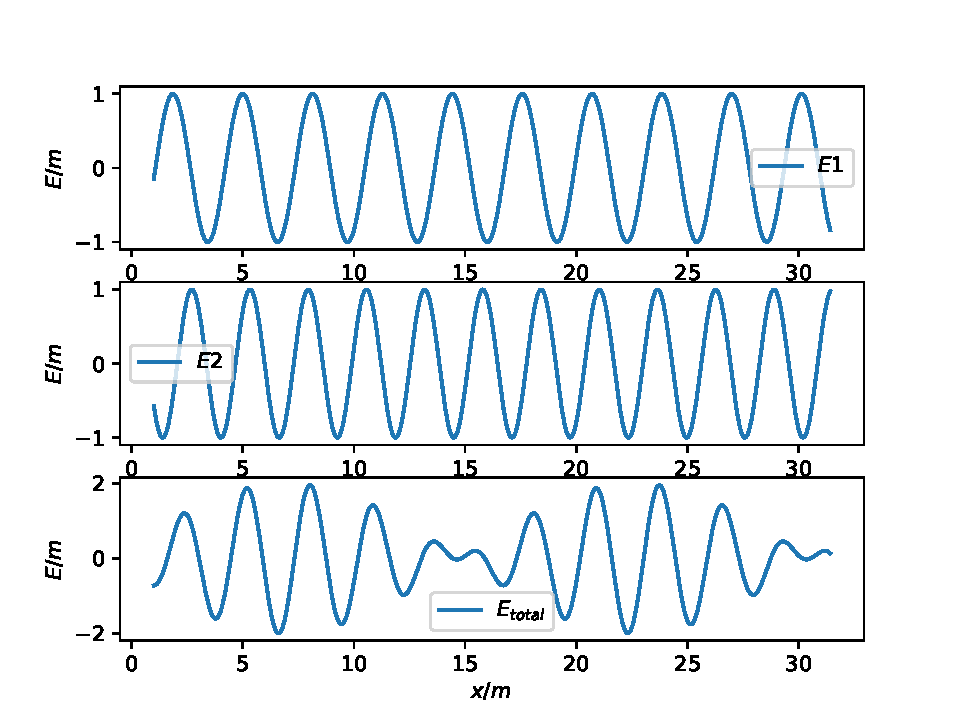
\includegraphics[width=0.9\linewidth]{image/beat.pdf}
    \caption{光拍频的形成}
    \label{fig:beat}
\end{figure}


我们用光电检测器接收这个拍频波。因为光电检测器的光敏面上光照所产生的光电流系光强 (即电场强度的平方)所引起, 故光电流为: $i_0=gE_s^2$.
 $g$  为接收器的光电转换常数。由于光频甚高 $ \left(f_{c}>10^{14} \mathrm{~Hz}\right)$ , 光敏面来不及 反映频率如此之高的光强变化, 迄今仅能反映频率  $10^{8} \mathrm{~Hz}$  左右的光强变化, 并产生光电流, 将 $ i_{c} $ 对时间积 分, 并取对光检测器的响应时间  $t\left(\frac{1}{f_{c}}<t<\frac{1}{\Delta f}\right)$  的平均值。结果,  $i_{c} $ 积分中高频项为零, 只留下常数项和缓 变项。即:
\begin{equation*}
    \left.\overline{i_{c}}=\frac{1}{t} \int_{i} \mathrm{id} t=g E^{2}\left\{1+\cos \left[\Delta \omega\left(t-\frac{x}{c}\right)+\Delta \varphi\right\rceil\right\}\right\}
\end{equation*}

其中 $ \Delta \omega$  是与  $\Delta f$  相应的角频率,  $\Delta \omega=2 \pi \Delta f, \Delta \varphi=\varphi_{1}-\varphi_{2} $ 为初相。可见光检测器输出的光电流包含有直流 和光拍信号两种成分。滤去直流成分, 即得频率为拍频 $ \Delta f$ , 相位与初相和空间位置有关的输出光拍信号。
图二是光拍信号 $ i_{c}$  在某一时刻的空间分布, 如果接收电路将直流成分滤掉, 即得纯粹的拍频信号在空 间的分布。这就是说处在不同空间位置的光检测器, 在同一时刻有不同相位的光电流输出, 这就提示我们 可以用比较相位的方法测定拍频波的波长, 进而测得光速。
事实上, 光拍频的同相位诸点有如下关系:\cite{钱建强2016近代物理实验}
\begin{equation}
    \Delta \omega \frac{x}{c}=2 n \pi \text { 或 } x=\frac{n c}{\Delta f}
\end{equation}

\subsection{相拍光束}
光拍频波产生要求相拍二光束具有一定的频差。使激光束产生频移的办法很多, 一种最常用的办法是 使超声与光波互相作用。声光相互作用产生三个效应: 声光调制、声光偏转和声光频移。在这里, 主要利 用了声光频移效应。
声光器件一端连接声光功率信号源, 引入高频信号; 另一端经 LC 匹配网 络将高频电信号加至与通光晶体紧贴的有铌酸锂材料做成的压 电换能器上 (有铵金电极的那一部分), 把高频电信号变成高频 声光信号在通光晶体里传播, 声波前进方向与光波前进方向相互 垂直, 声子与光子相互碰撞, 产生声光效应。为了有较高的衍射 效率, 通光晶体选用了钽酸铅材料。\cite{安毓英2003光电子技术}

利用声光相互作用产生频移的方法有二。一是行波法, 在声光介质与声源 (压电换能器) 相对的端面 上敷以吸声材料或做成牛角形, 防止声反射, 以保证只有声行波通过, 如图\ref{fig:介质}所示。声光器件没加电信号 时, 激光穿过晶体, 入射光与穿过晶体的出射光在频率上没有变化, 也没有衍射现象产生。当声光器件加 上电信号时, 经压电换能器电信号变成同频率的超声波 (弹性波) 在与光束前进方向相垂直的方向上传播, 引起通光晶体光折射率发生周期性变化, 形成一相位光栅 (体光棚), 出射光束不仅发生衍射现象, 频率 上也发生了与声频有光的频移。第  $l $ 级衍射光的角频率为:  $\omega_{l}=\omega_{0}+l \Omega $ 。其中 $ \omega_{0}$  为入射光的角频率,  $\Omega  $为 声角频率, 衍射级 $ l=\pm 1, \pm 2, \cdots$ , 如其中  +1  级衍射光频为  $\omega_{0}+\Omega $, 衍射角为  $\alpha=\frac{\lambda}{\Lambda}, \lambda$  和  $\Lambda$  分别为介质中的光和声波长。通过仔细的光路调节, 我们可使  +1  级与 0 级二光束平行迭加, 产生频差为 $ \Omega$  的光拍频 波。
另一种是驻波法, 如图五所示。利用声波的反射, 使介质中存在驻波声场 (相应于介质传声的厚度为 半声波长的整数倍的情况)。它也产生  $l$  级对称衍射, 而且衍射光比行波法时强得多 (衍射效率高), 第  $l$  级的衍射光频为:

\begin{equation}
    \omega_{l, m}=\omega_{0}+(l+2 m) \Omega
\end{equation}

其中 $ l, m=0, \pm 1, \pm 2, \cdots ,$ 可见在同一级衍射光束内就含有许多不同频率的光波的迭加(当然强度不相 同), 因此用不到光路的调节就能获得拍频波。例如选取第一级, 由  m=0  和  +1  的两种频率成分迭加得到 拍频为 $ 2 \Omega$  的拍频波。
两种方法比较, 显然驻波法有利, 我们就此选择驻波型声光器件来产生 2 倍于声频的光拍频波。由于 驻波法有倍频效应, 在实验时, 必须将频率计的读数  $\times 2  $才是光拍频波的真实频率。\cite{安毓英2003光电子技术}

\subsection{声光法测量声速}
显然, 由驻波条件:
式中  m  为正整数, $ \Lambda $ 为超声波长,$  \Lambda=v / f, v$  为声速,  $f $ 为功率源频率, 

\begin{equation}\label{d}
    d=m \frac{v}{2 f}  \\
    f=m \frac{v}{2 d} 
\end{equation}

由\ref{d}式可知, 当  $d $ 一定时, 可以在通光介质中形成不同频率的驻声波场, 其  $m$  数由声频 $ f$  确定。 当光束垂直驻波场入射时将产生 Raman-Nath 衍射, 在换能器频率响应带宽 $ \Delta f $ 范围内调节频率 $ f$ , 可找到 不同个 $ m$  值对应于衍射效应最强点 (衍射级数最多, 即衍射点数最多处), 而衍射效应最强点之间则有暗 的过渡。

\begin{figure}
    \centering
    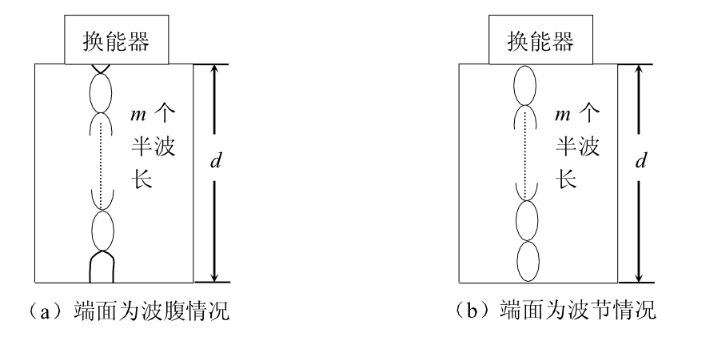
\includegraphics[width=\linewidth]{image/声光介质.png}
    \caption{声光介质中形成驻波衍射光栅}
    \label{fig:介质}
\end{figure}

\section{实验数据}
测量开始前,得到频率 $f_1=74.9990 \mathrm{Hz}$ 结束是频率$f_2=74.9979 \mathrm{Hz}$,此时波的周期为 $T=2.235 \mu s$,固定一个小车与 $x_0=2.00cm$处,记录另一组小车位置:
\begin{table}[h]
\centering
\captionnamefont{\wuhao\bf\heiti}
\captiontitlefont{\wuhao\bf\heiti}
\caption{光程差和频率的关系} \label{tab:eg2}
\liuhao
\begin{tabular}{|c|c|c|c|}
\hline
 &x/cm & $\Delta t / \mu s$ & D/cm   \\ \hline
1 &\textit{4.00} & \textit{0.180} & \textit{2.00}  \\ \hline
2 &\textit{8.00} & \textit{0.255} & \textit{6.00}  \\ \hline
3 &\textit{12.00} & \textit{0.315} &\textit{10.00}  \\ \hline
4 &  \textit{16.00} &\textit{0.405} &\textit{14.00} \\ \hline
5 & \textit{20.00} &\textit{0.515} &\textit{18.00}  \\ \hline
6&  \textit{24.00} &\textit{0.570} &\textit{22.00}  \\ \hline
7&  \textit{28.00} &\textit{0.655} &\textit{26.00} \\ \hline
8&  \textit{32.00} &\textit{0.745} &\textit{30.00} \\ \hline
\end{tabular}
\end{table}

从LM2000C声光器件上标定读书声光介质厚度 $d=8.47mm$,在换能器频响带宽 $\Delta f$范围内调节频率 $f$,通过判别衍射效应最强点之间暗 的过渡,可以找到不同m值对应的衍射最强点,起始频率为 $f_1=74.4772 \mathrm{MHz}$ 记录下每次变化时的频率:

\begin{table}[h]
\centering
\captionnamefont{\wuhao\bf\heiti}
\captiontitlefont{\wuhao\bf\heiti}
\caption{明暗变化时的频率 $f/\mathrm{MHz}$ } \label{tab:eg2}
\liuhao
\begin{tabular}{|c|c|c|c|}
\hline
 f_2=74.6874 & f_3=74.9207 & f_4=75.1105 &f_5=75.3246 \\
 f_6=75.5369 &f_7=75.7473 &f_8=75.9600 & f_9=76.1724 \\
\hline
\end{tabular}
\end{table}

然后将透明介质水放于轨道上,移动小车使得外光路与内光路曲线重合,将小车A放于 $x_1=53.00cm$的位置,记录得到小车B的位置:
\begin{table}[h]
\centering
\captionnamefont{\wuhao\bf\heiti}
\captiontitlefont{\wuhao\bf\heiti}
\caption{明暗变化时的频率 $f/\mathrm{MHz}$ } \label{tab:eg2}
\liuhao
\begin{tabular}{|c|c|c|}
\hline
 &初始位置/cm &结束位置/cm \\
1& 57.40&42.00 \\
2&56.80 & 41.95 \\
3& 57.50& 42.15 \\
4& 56.70& 42.40 \\
5& 56.70& 41.50 \\
\hline
\end{tabular}
\end{table}

\section{实验结果分析}
通过第一个表拟合出来:
$$D=49.022 \times 10^4 m/s \Delta t -6.305 m$$
最终得到光速 $c=3.18 \pm 0.005 \times 10^8 m/s$ 得到$ \delta f=1.6952 \mathrm{MHz}$,声光介质中声速为 $V=2d \delta f =3589.586 m/s$。最后测量得到 $\Bar{\Delta x}= 15.02cm$,水管长度 $42cm$ 折射率为 $1+\frac{\Bar{\Delta x}}{L}=1.357$



\section{结~~论}
本实验利用LM2000C 型光速测量仪和光电接收器分别用光拍法测量光速和声光法测量透明介质中的声速,了解了声光效应的Raman-Nath衍射的概念测量得到光速为 $c==3.18 \pm 0.005 \times 10^8 m/s$,介质声速$v=3589.586 m/s$ 最后利用光拍法补偿法测量水的折射率 $n=1.357$。


%%%%%%%%%%%%%%%%%%%%%%%%%%%%%%%%%%%%%%%%%%%%%%%%%%%%%%%%%%%%%%%%
%  参考文献
%%%%%%%%%%%%%%%%%%%%%%%%%%%%%%%%%%%%%%%%%%%%%%%%%%%%%%%%%%%%%%%%
%  参考文献按GB/T 7714-2015《文后参考文献著录规则》的要求著录. 
%  参考文献在正文中的引用方法:\cite{bib文件条目的第一行}

\renewcommand\refname{\heiti\wuhao\centerline{参考文献}\global\def\refname{参考文献}}
\vskip 12pt

\let\OLDthebibliography\thebibliography
\renewcommand\thebibliography[1]{
  \OLDthebibliography{#1}
  \setlength{\parskip}{0pt}
  \setlength{\itemsep}{0pt plus 0.3ex}
}

{
\renewcommand{\baselinestretch}{0.9}
\liuhao
\bibliographystyle{gbt7714-numerical}
\bibliography{./TempExample}
}


\end{document}
